\ppageno=15
\ppreviouspageno=14
\plineno=39
\psublineno=1

\newParkoszpage

{\relsize{-2}
\url{http://ebuw.uw.edu.pl/Content/215606/directory.djvu?djvuopts=&page=55&zoom=width&showposition=0.5,0.18}

\url{http://ebuw.uw.edu.pl/Content/215606/directory.djvu?djvuopts=&page=78&zoom=width&showposition=0.5,0.81}
}

\bigskip

\obeylines
\mono



\fullpreviouslines


{
\color{blue}

Tamen

eciam in suis locis possemus singulas predictas
}

\plineno=0

\fulllines

litteras seu earum exempla ponere, sicut et ponemus. Non

est enim vicium idem pluries repetere ex causa notandum.

% \def\splitlines{\advance\plineno by 1\psublineno=0\everypar{\advance\psublineno by 1\llap{\textcolor{green}{\the\ppageno-\ifnum\plineno<10 0\fi\the \plineno-\the\psublineno \ }}}}

% \def\newsplitline{\advance\plineno by 1}

\def\splitverse{\advance\plineno by 1\psublineno=0\everypar{\advance\psublineno by 1\llap{\textcolor{green}{\the\ppageno-\ifnum\plineno<10 0\fi\the \plineno-\the\psublineno \ }}\hskip5em}}

% nie działa licznik wierszy?
\def\fullverselines{\everypar{\advance\plineno by 1\llap{\the\ppageno-\ifnum\plineno<10 0\fi\the \plineno \hskip 1.5em}\hskip5em}}


\def\newverse{\advance\plineno by 1\psublineno=0\hskip10em}
\def\newversesubline{\hskip\indentV}
\def\newverseline{\advance\plineno by 1\psublineno=0}
\newdimen\indentV
\newdimen\indentVt
\indentV=5em
%\setlength{\indentV}{10em}
\def\indentVerse{\hskip\indentV{}}
\def\indentVerseTotal{\hskip\indentVt{}}

% MUFI SHORT VIRGULA
% skomentowac w artykule!

{

\catcode`\/=13
\def/{{\fontCardo }}

% 
\includegraphics[width=\hsize]{wierszP1m}

\splitverse

%\indentVerse
\parkosz{Ktho} \parkosz{chce} \parkosz{piſſaç} \parkosz{doſkoɲaɬe}

%\indentVerse
\parkosz{Ġøzik} \parkosz{poɬſki}

% 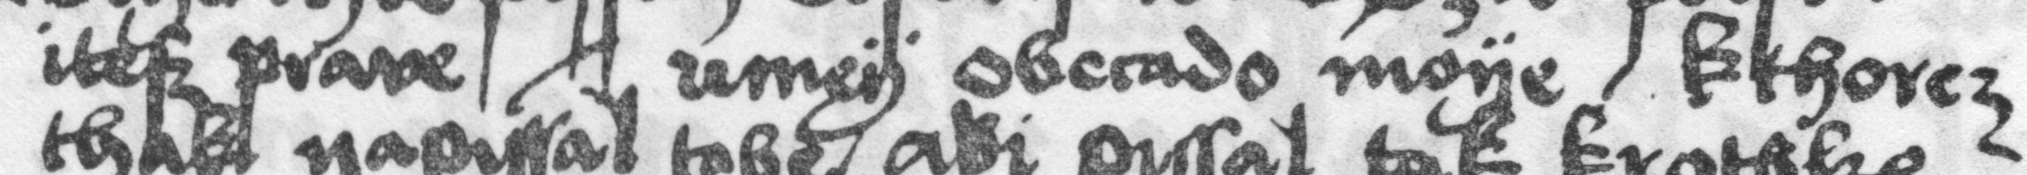
\includegraphics[width=\hsize]{wierszP2}

%\newverse
\splitverse

\settowidth{\indentV}{\parkosz{Ġøzik} \parkosz{poɬſki}}
\indentVerse \parkosz{itefz} \parkosz{prave}/

% \indentVerse
\parkosz{uṃeÿ} \parkosz{obecado} \parkosz{ṃoÿe}/

% http://en.wikipedia.org/wiki/Ezh
% 'LATIN SMALL LETTER EZH' (U+0292)
	
\catcode `\^^M=5
\newtip{85}{Tak w rkp., z pewnością należy czytać \textit{ktorem}, a nie \textit{któreż}, co jednak
nie jest o tyle pewne, że w wyrazach, polskich w traktacie skrótów nie ma.}
\obeylines

% \indentVerse
\parkosz{kthore\conf{ʒ}{}}¹

% 85 Tak w rkp., z pewnością należy czytać Morem, a nie któreś, Co jednak

% nie jest o tyle pewne, że w wyrazach, polskich w traktacie skrótów nie ma.

% 
\includegraphics[width=\hsize]{wierszP3}


\splitverse

\settowidth{\indentV}{\parkosz{kthore\conf{ʒ}{}}}
\indentVerse \parkosz{thak} \parkosz{ɲapiſſaḷ} \parkosz{toɓe}/

\parkosz{aɓi} \parkosz{piſſaḷ} \parkosz{tak} \parkosz{krothke}

% 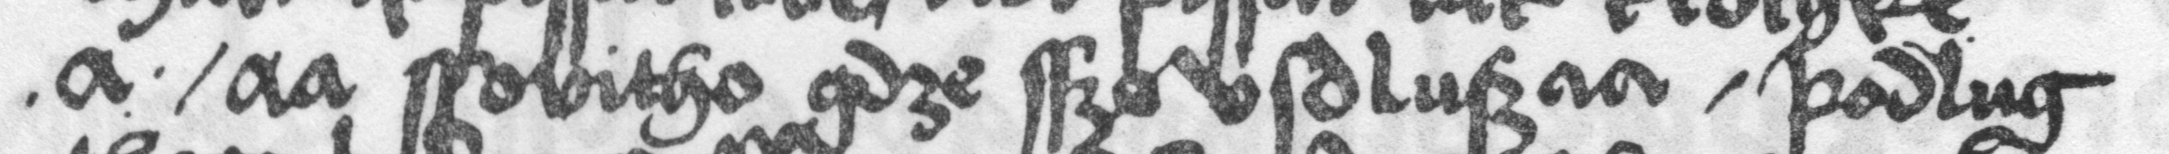
\includegraphics[width=\hsize]{wierszP4}

\splitverse

\settowidth{\indentV}{\parkosz{aɓi} \parkosz{piſſaḷ} \parkosz{tak} \parkosz{krothke}}
\indentVerse · \parkosz{a} ·/

\parkosz{\textit{aa}} \parkosz{ſſovitho} \parkosz{ꝿdze} \parkosz{ſſzø} \parkosz{ʋſdḷuſzaa}/

\parkosz{podḷuꝿ}

% 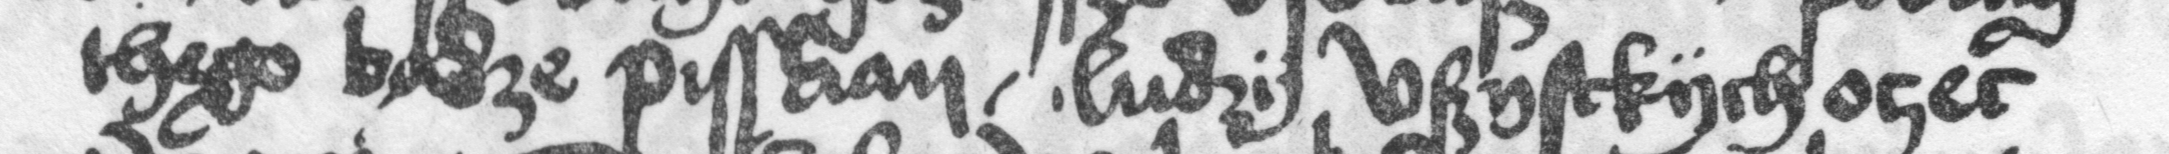
\includegraphics[width=\hsize]{wierszP5}

\splitverse

\settowidth{\indentV}{\parkosz{podḷuꝿ}}
\indentVerse \parkosz{theꝿo} \parkosz{bødze} \parkosz{piſſaaɲ}/


\parkosz{ɬudzij} \parkosz{ʋſzyſtkijch} \parkosz{oçec}

% 
\includegraphics[width=\hsize]{wierszP6}

\splitverse

\settowidth{\indentV}{\parkosz{ɬudzij} \parkosz{ʋſzyſtkijch} \parkosz{oçec}}
\indentVerse \parkosz{\textit{adaaɱ}}/

%\settowidth{\indentV}{\parkosz{\textit{adaaɱ}}/}
%\indentVerse
\parkosz{A} \parkosz{theſz ġdze} · \parkosz{ƀ} · \parkosz{bødze} \parkosz{ġruube}/

% \newverseline

% 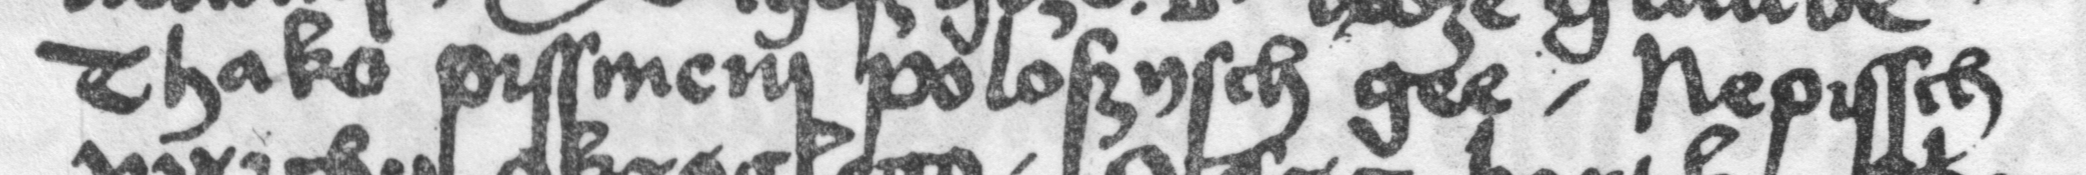
\includegraphics[width=\hsize]{wierszP7}

\splitverse

\parkosz{Thako} \parkosz{piſſṃeɱ} \parkosz{poḷoſzyſch} \parkosz{ġee}/

%\settowidth{\indentV}{\parkosz{Thako} \parkosz{piſſṃeɱ} \parkosz{poḷoſzyſch} \parkosz{ġee}/}
%\newversesubline
\parkosz{Ṇepiſſch}

% 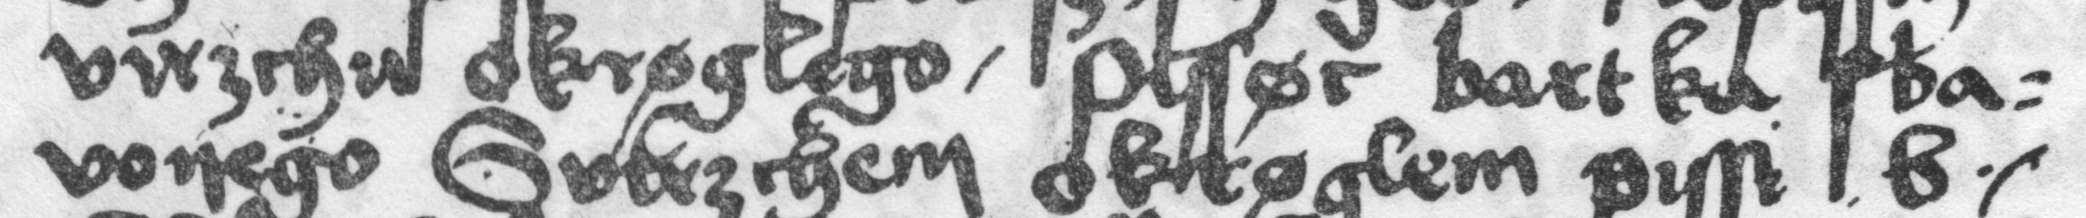
\includegraphics[width=\hsize]{wierszP8}

\settowidth{\indentV}{\parkosz{Ṇepiſſch}}
\splitverse
\indentVerse \parkosz{virzchu} \parkosz{okrøꝿɬeꝿo}/

%\settowidth{\indentV}{\parkosz{virzchu} \parkosz{okrøꝿɬeꝿo}/}
\parkosz{Piſſøc} \parkosz{\textit{bartka}} \parkosz{\textit{\hyphh{ſba}{voɲeġo}}}

% 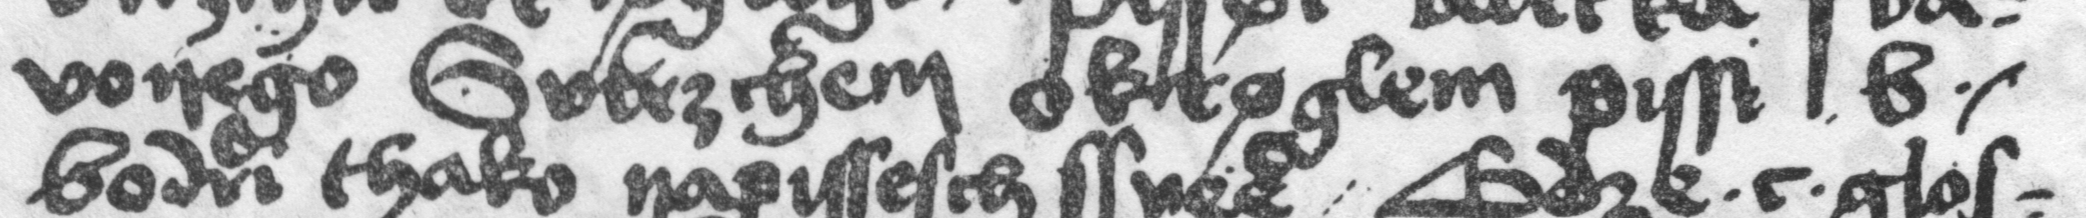
\includegraphics[width=\hsize]{wierszP9}

%\newverseline
\fullverselines

 \parkosz{\textit{\hypht{ſba}{voɲeġo}}} \parkosz{Svirzcheɱ} \parkosz{okrøꝿɬeṃ} \parkosz{piſſi} · \parkosz{ɓ} ·/

% 
\includegraphics[width=\hsize]{wierszP10}

\plineno=11
\splitverse

\parkosz{\textit{ɓodri}} \parkosz{thako} \parkosz{ɲapiſſeſch} \parkosz{ſſvee}/

% zły numer!

%\settowidth{\indentV}{\parkosz{\textit{ɓodri}} \parkosz{thako} \parkosz{ɲapiſſeſch} \parkosz{ſſvee}/}
%\indentVerse
\parkosz{Ġdze} · \parkosz{\textit{c}} · \parkosz{\hyphh{ġḷoſ}{ſu}}

% 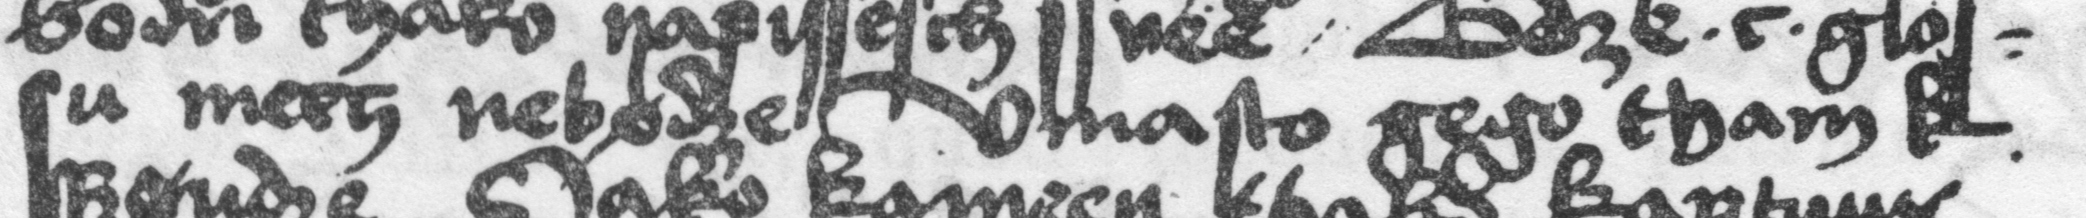
\includegraphics[width=\hsize]{wierszP11}

\splitverse

\settowidth{\indentV}{\parkosz{Ġdze} · \parkosz{\textit{c}} · \parkosz{\hyphh{ġḷoſ}{}}}
\indentVerse \parkosz{\hypht{ġḷoſ}{ſu}} \parkosz{ṃeeç} \parkosz{ṇebødze}

%\settowidth{\indentV}{\parkosz{\hypht{ġḷoſ}{ſu}} \parkosz{ṃeeç} \parkosz{ṇebødze}}
% \indentVerse
\parkosz{Vṃaſto} \parkosz{ġeꝿo} \parkosz{thaṃ} \parkosz{\textit{k}}

% 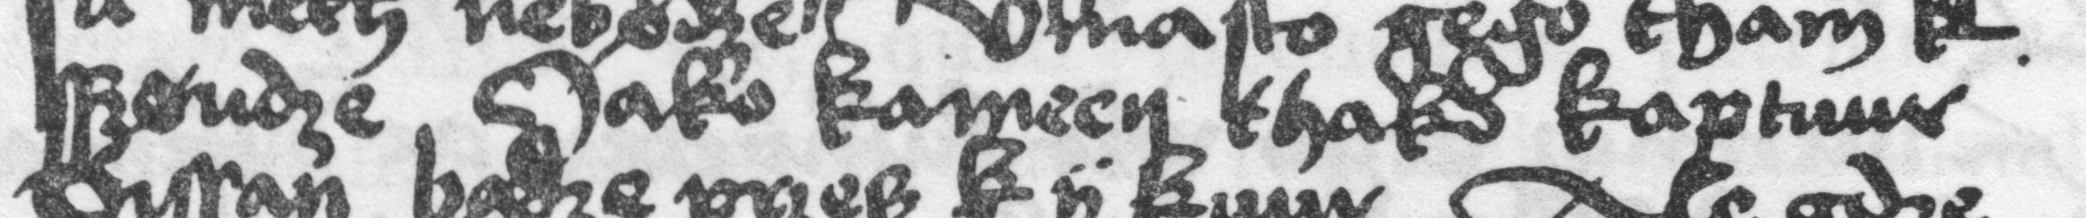
\includegraphics[width=\hsize]{wierszP12}

\splitverse

\settowidth{\indentV}{\parkosz{Vṃaſto} \parkosz{ġeꝿo} \parkosz{thaṃ} \parkosz{\textit{k}}}
 \indentVerse \parkosz{ſſzøṇdze}

\parkosz{Iako} \parkosz{\textit{kaṃeeɲ}} \parkosz{thako} \parkosz{\textit{kaᵽtuur}}

\newpage
% 
\includegraphics[width=\hsize]{wierszP13}

\splitverse

% brak Ƥ
\parkosz{Ƥiſſaɲ} \parkosz{bⱥdze} \parkosz{przes} \parkosz{\textit{k}} \parkosz{ÿ} \parkosz{\textit{kuur}}

% \indentVerse
\parkosz{Aɬe} \parkosz{ꝿdze}

% 
\includegraphics[width=\hsize]{wierszP14}

\splitverse

\settowidth{\indentV}{\parkosz{Aɬe} \parkosz{ꝿdze}}
 \indentVerse · \parkosz{\textit{c}} · \parkosz{ſvoij} \parkosz{ꝿḷos} \parkosz{ṃeʋa}

 %\indentVerse
 \parkosz{Svikḷeṃ} \parkosz{pijſṃeɱ}

% 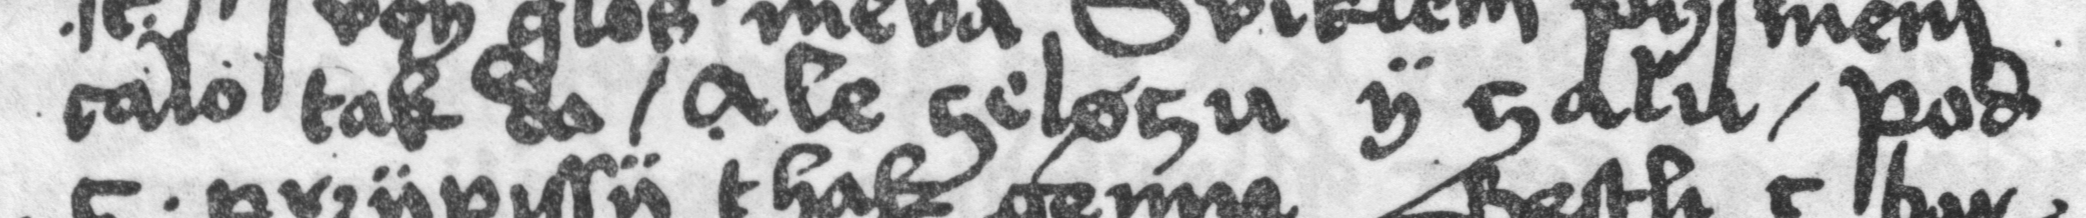
\includegraphics[width=\hsize]{wierszP15}

\splitverse

\settowidth{\indentV}{\parkosz{Svikḷeṃ} \parkosz{pijſṃeɱ}}
\indentVerse \parkosz{caḷo} \parkosz{tak} \parkosz{da}/

%\indentVerse
\parkosz{Aɬe} \parkosz{\textit{çeløçu}} \parkosz{ÿ} \parkosz{\textit{çalu}}/

\parkosz{pod}

% 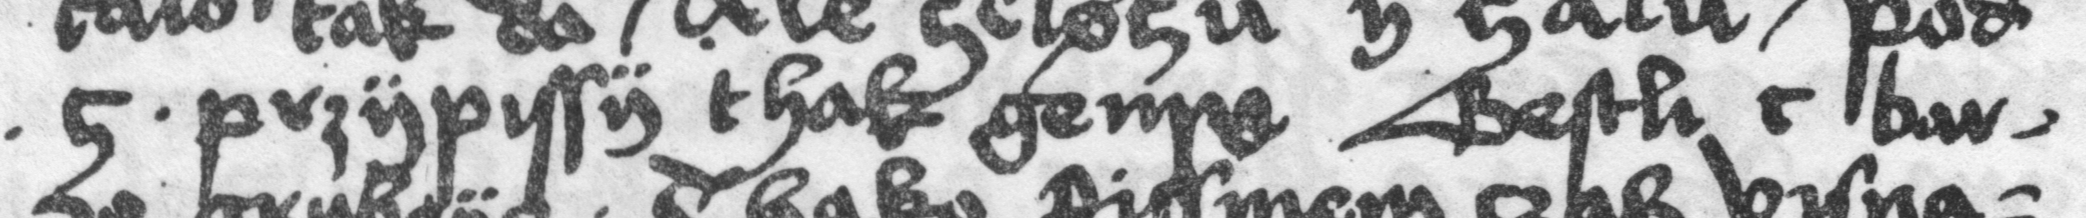
\includegraphics[width=\hsize]{wierszP16}

\splitverse

\settowidth{\indentV}{\parkosz{pod}}
\indentVerse · \parkosz{ç} · \parkosz{przÿpiſſy} \parkosz{thak} \parkosz{ġeɱv}

%\indentVerse
\parkosz{Ġeſtɬi} \parkosz{\textit{c}} \parkosz{\hyphh{bar}{zo}}

% 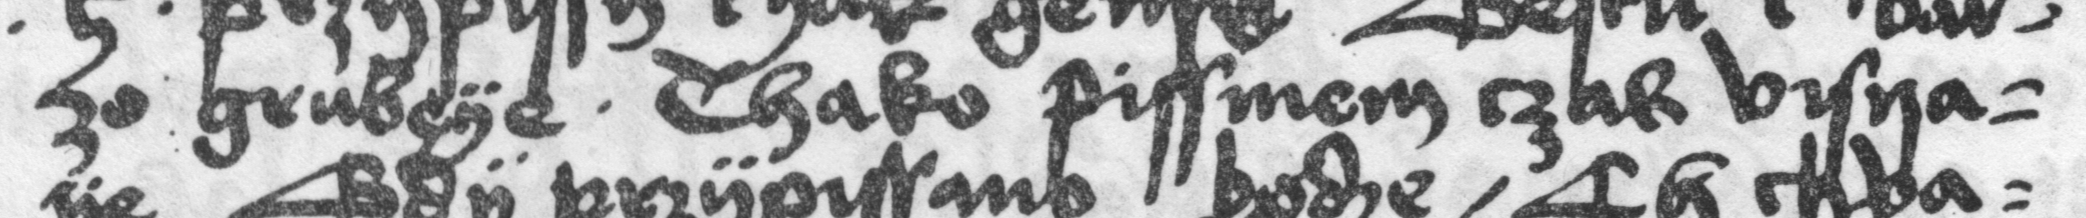
\includegraphics[width=\hsize]{wierszP17}

\settowidth{\indentV}{\parkosz{Ġeſtɬi} \parkosz{\textit{c}} \parkosz{\hyphh{bar}{}}}
\indentVerse  \parkosz{\hypht{bar}{zo}} \parkosz{ġruɓeÿe}.

\parkosz{Thako} \parkosz{piſſṃeṃ} \parkosz{\textit{czas}} \parkosz{\hyphh{ʋiſɲa}{ÿe}}

% 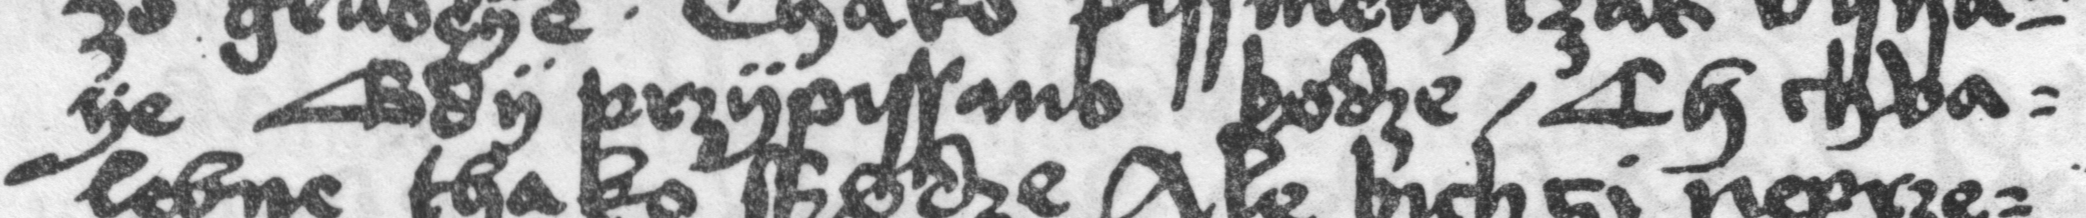
\includegraphics[width=\hsize]{wierszP18}
\settowidth{\indentV}{\parkosz{Thako} \parkosz{piſſṃeṃ} \parkosz{\textit{czas}} \parkosz{\hyphh{ʋiſɲa}{}}}
\indentVerse \parkosz{\hypht{ʋiſɲa}{ÿe}}

\parkosz{Ġdy} \add{h} \parkosz{przijpiſſaṇo} \parkosz{bødze}/

\parkosz{\textit{Ch}}  \parkosz{\hyphh{chʋa}{ɬebɲe}}

%\newpage

% 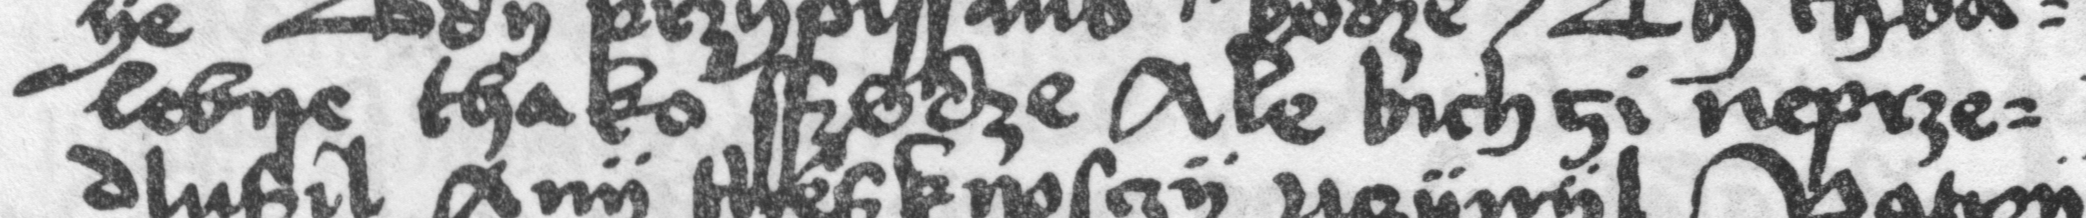
\includegraphics[width=\hsize]{wierszP19}

\splitverse

\settowidth{\indentV}{\parkosz{\textit{Ch}}  \parkosz{\hyphh{chʋa}{}}}
\indentVerse \parkosz{\hypht{chʋa}{ɬebɲe}} \parkosz{thako} \parkosz{ſſzødze}

% \indentVerse
\parkosz{Aɬe} \parkosz{bich} \parkosz{çi} \parkosz{\hyphh{ṇeprze}{dḷuſziḷ}}

% 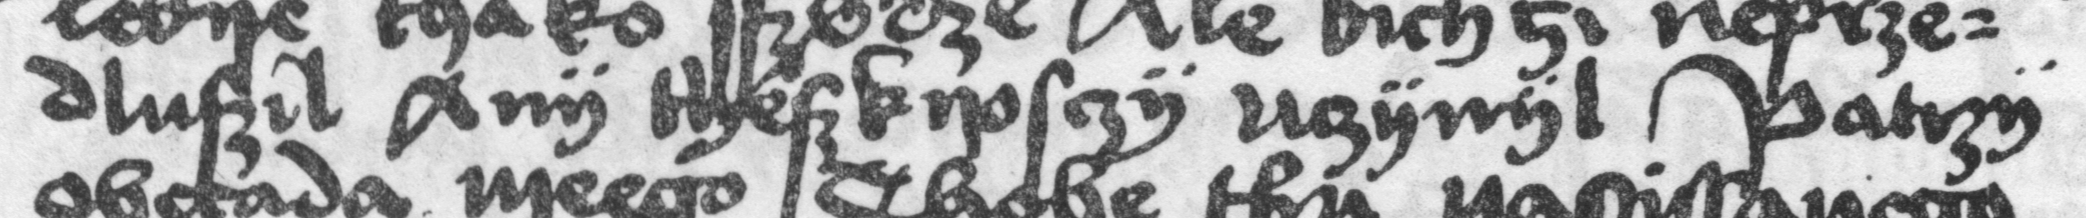
\includegraphics[width=\hsize]{wierszP20}

\splitverse

\settowidth{\indentV}{\parkosz{Aɬe} \parkosz{bich} \parkosz{çi} \parkosz{\hyphh{ṇeprze}{}}}
\indentVerse \parkosz{\hypht{ṇeprze}{dḷuſziḷ}}

\parkosz{Aṇÿ} \parkosz{theſzkɲoſczÿ} \parkosz{uczÿṇÿḷ}

%\indentVerse
\parkosz{Patrzÿ}

% 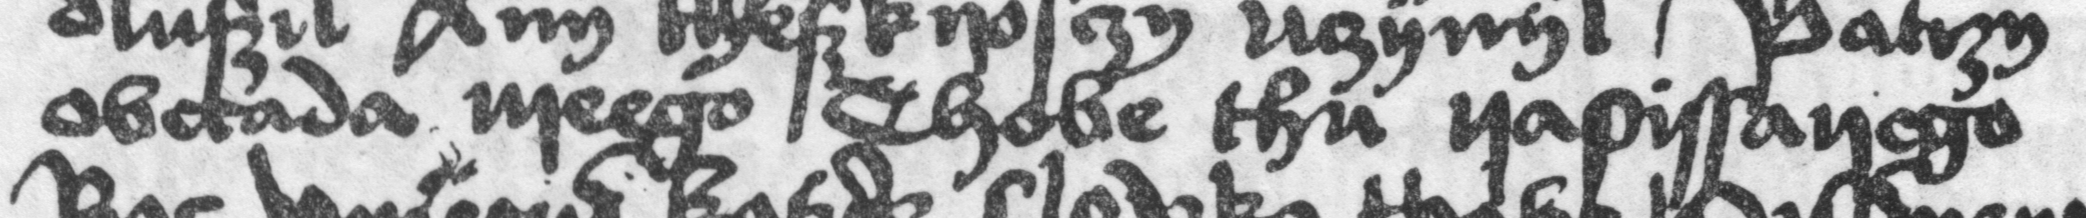
\includegraphics[width=\hsize]{wierszP21}

\splitverse

\settowidth{\indentV}{\parkosz{Patrzÿ}}
\indentVerse \parkosz{obecada} \parkosz{ɱeeġo}

%\indentVerse
\parkosz{Thoɓe} \parkosz{thu} \parkosz{ɲapiſſaɲeġo}

% 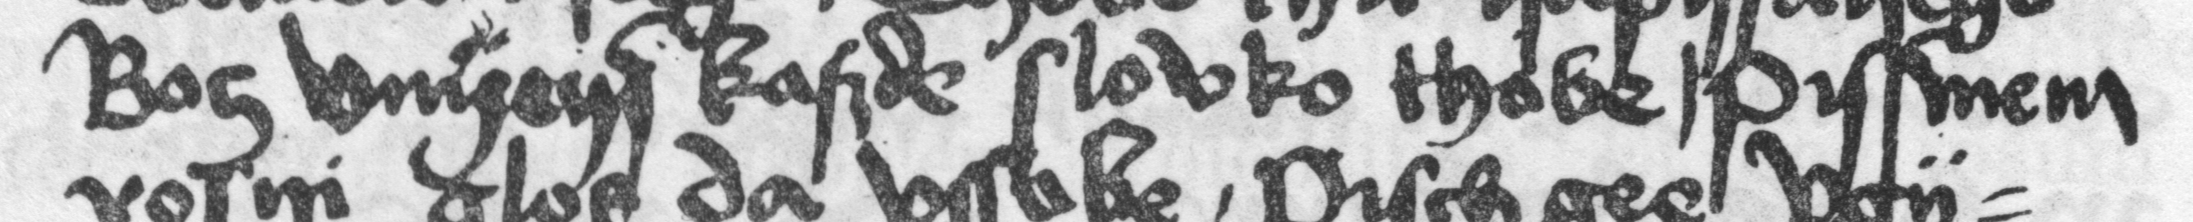
\includegraphics[width=\hsize]{wierszP22}

\splitverse

\parkosz{Boç} \parkosz{ʋṇye\conf{ɱ}{}} \parkosz{kaſzde} \parkosz{ſḷoʋko} \parkosz{thobe} /

% \indentVerse
\parkosz{Ƥiſſṃeɱ}

% 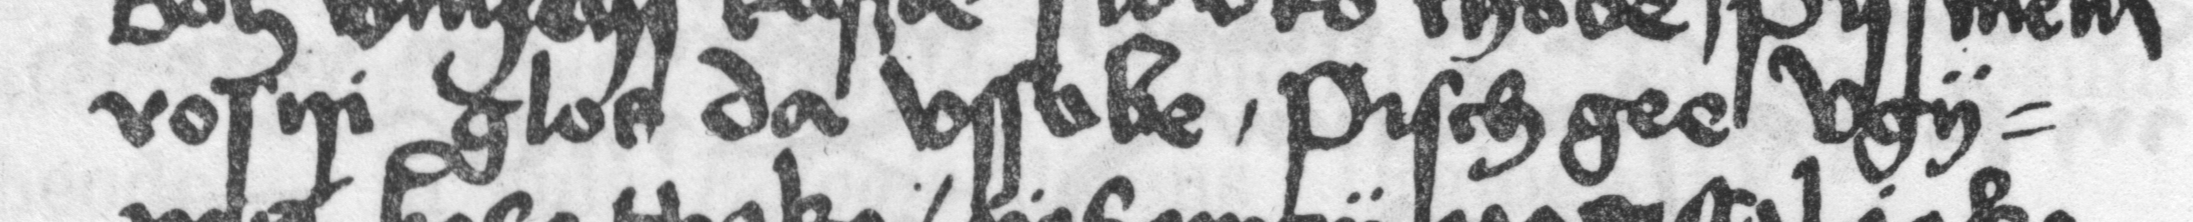
\includegraphics[width=\hsize]{wierszP23}

\splitverse

\settowidth{\indentV}{\parkosz{Ƥiſſṃeɱ}}
\indentVerse \parkosz{roſɲi} \parkosz{ġḷos} \parkosz{da} \parkosz{ʋſſobe}/

\parkosz{Piſch} \parkosz{ġee} \parkosz{\hyphh{Vġij}{ṃo}}

% 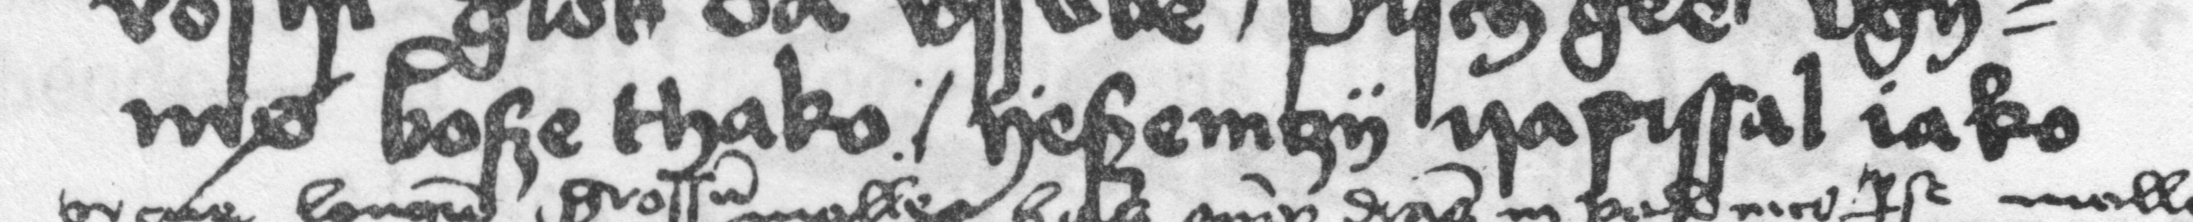
\includegraphics[width=\hsize]{wierszP24}

\splitverse

\settowidth{\indentV}{\parkosz{Piſch} \parkosz{ġee} \parkosz{\hyphh{Vġij}{}}}
\indentVerse \parkosz{\hypht{Vġij}{ṃo}} \parkosz{boſze} \parkosz{thako}/

\catcode `\^^M=5
\newtip{86}{Nie sygnalizujemy pisowni w wielu wypadkach niezgodnej z
  zaleceniami. Cały ten wiersz w pisowni zrekonstruowanej według
  wskazówek Parkosza ogłosił Łoś w Języku Polskim I, 1913, s. 56.}
\obeylines
\parkosz{ijeſzeṃczij} \parkosz{ɲapiſſaḷ} \parkosz{iako}¹
% •* Nie sygnalizujemy pisowni w wielu wypadkach niezgodnej z zale¬

% ceniami. Cały ten wiersz w pisowni zrekonstruowanej według wskazówek

% Parkosza ogłosił Łoś w Języku Polskim I, 1913, s. 56.

% koniec wiersza!!!

\newpage

\splitlines

% 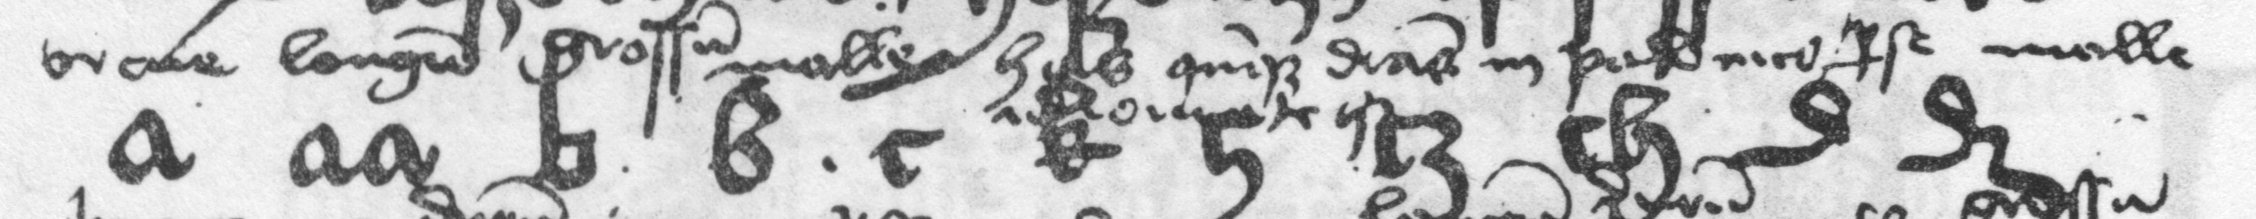
\includegraphics[width=\hsize]{wierszP25-26}


breue \parkosz{a} 

longum \parkosz{aa} 

groſſum \parkosz{ƀ} 

molle \parkosz{ɓ} 

\parkosz{c} has quinque differencias in Polonico idiomate habet \parkosz{c} \parkosz{k} \parkosz{ç} \parkosz{cz} \parkosz{ch}

per ſe \parkosz{d} 

molle \parkosz{dz} 

breue \parkosz{e} 

longum \parkosz{ee} 

durum \parkosz{ff} 

molle \parkosz{ḟ} 

% 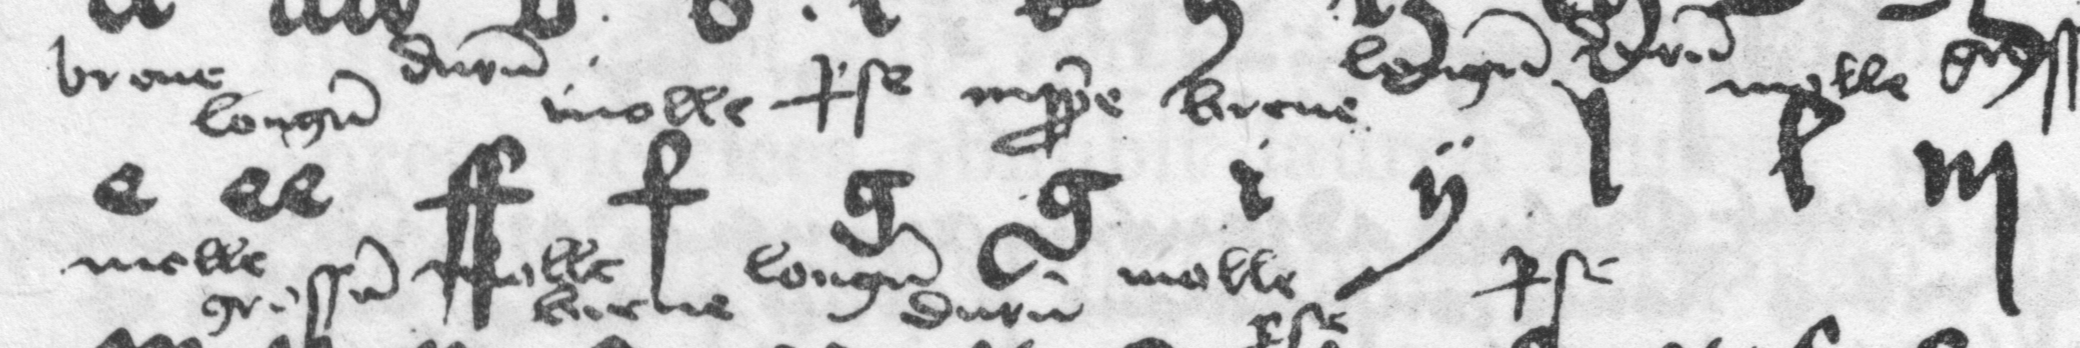
\includegraphics[width=\hsize]{wierszP27-28}



\newtip{87}{Winno być: per se \parkosz{ꝿ}, improprie \parkosz{ġ}.}
per ſe \parkosz{ġ} 

inproprie \parkosz{ꝿ}¹  
% 87	Winno być: per se g, improprie g.

breue \parkosz{i} 

longum \parkosz{ij} 

durum \parkosz{ḷ} 

molle \parkosz{ɬ} 

groſſum \parkosz{ɱ} 

molle \parkosz{ṃ} 

groſſum \parkosz{ɲ}  

molle \parkosz{ṇ}   

breue \parkosz{o} 

longum \parkosz{oo} 

% 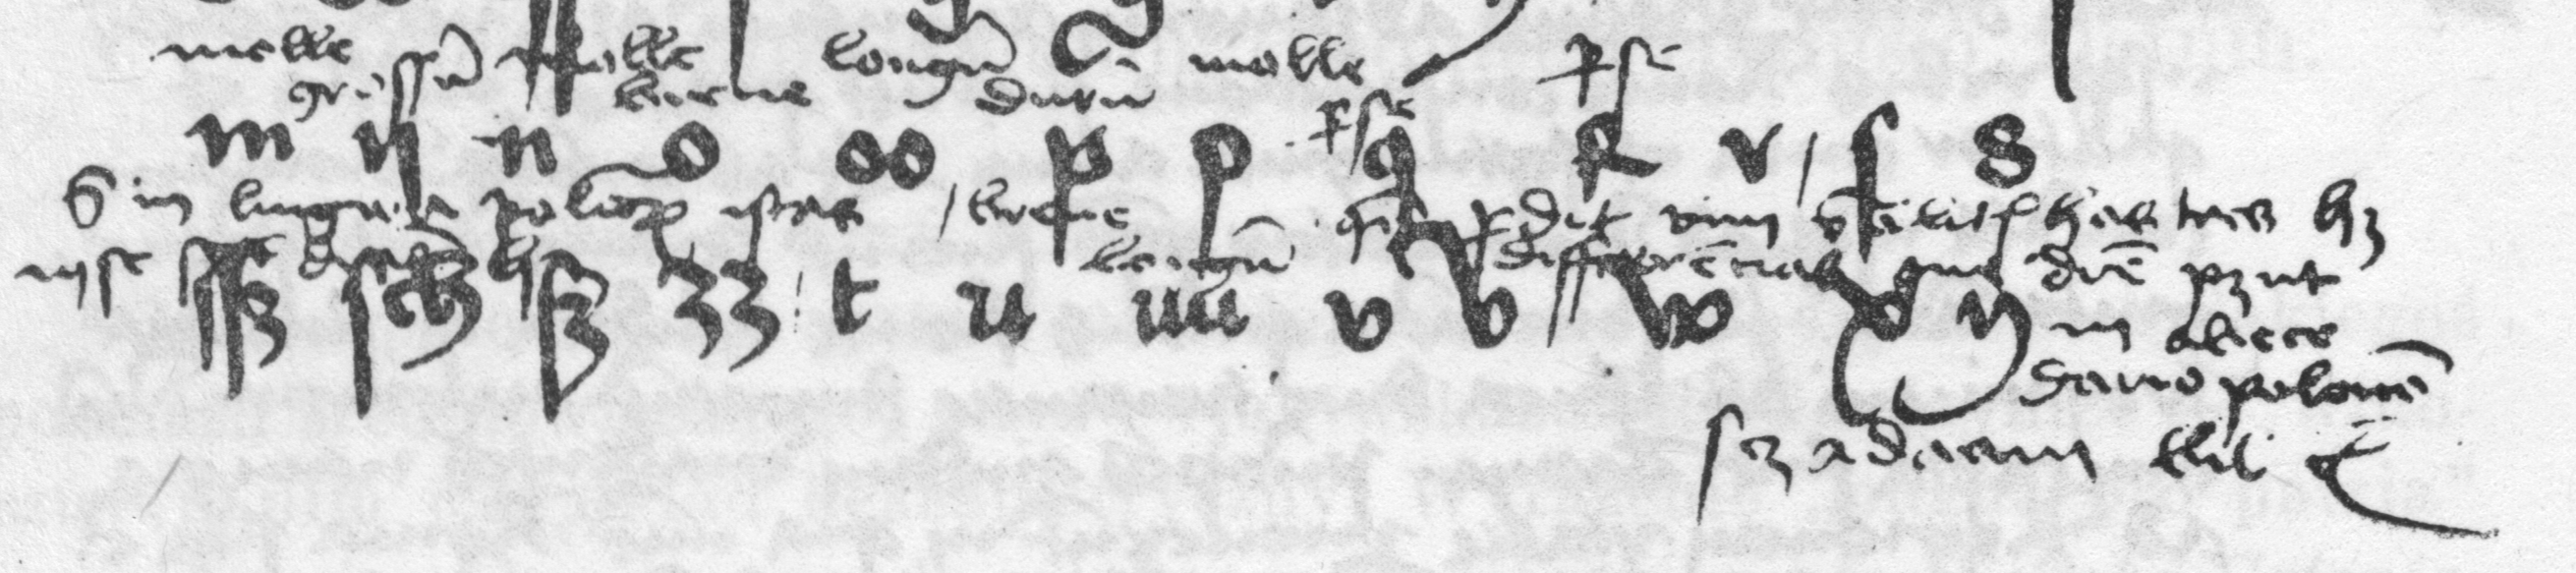
\includegraphics[width=\hsize]{wierszP29-koniec}


durum \parkosz{ᵽ} 

molle \parkosz{ƥ} 

per ſe \parkosz{q} 

per ſe \parkosz{R} \parkosz{r}


\parkosz{S} in lingua Polonorum iſtas in ſe ſex differencias habet \parkosz{ſ} \parkosz{s} \parkosz{ſſz} \parkosz{ſch} \parkosz{ſz} \parkosz{zz}

\parkosz{t}

breue \parkosz{u} 

longum \parkosz{uu} 

cum perdit vim vocalitatis, has tres habet differencias, que differencie patent in abecedario Polonorum, {ſcilicet} \parkosz{adaam} \parkosz{ɓiɬ} etc. \parkosz{v} \parkosz{ʋ} \parkosz{w}

\parkosz{x}

\parkosz{y}



\endinput



% \fullfines

% \ppreviouspageno=16
% \plineno=0


% \fullpreviouslines


% {
% \color{blue}

% ???


% }




% \endinput


%%%%%%%%%%%%%%%%%%%%%%%%%%%%%%%%%%%%%%%%%%%%%%%%%%%%%%%%%%%%%%%%%%%%%%%%%%%%%%%%%%%%%%%%%%%




\catcode `\^^M=5

  \newtip{48}{Łoś niesłusznie uważa, że \textit{bika} w obu wypadkach
    napisano błędnie zamiast \textit{ƀyka}. Przykłady są bowiem podane
    w~pisowni dotychczasowej dla pokazania jej niewystarczalności do
    zróżnicowania wyrazów \textit{bika} i \textit{byka}.}

\obeylines






\newcommand{\margin}[1]{\annotatetextBlue{\{#1\}}{zapisy na marginesie}}


% \renewcommand{\over}[1]{\colorbox{blue!10}{\{#1\}}}

\renewcommand{\over}[1]{\annotatetextBlue{\{#1\}}{zapisy nad rządkami}}

% litery i wyrazy dodane, (których w tekście brak)
%\newcommand{\add}[1]{\colorbox{olive!10}{<#1>}}
\newcommand{\add}[1]{\annotatetextOlive{<#1>}{litery i wyrazy dodane, (których w tekście brak)}}

% litery i wyrazy zbędne
% \newcommand{\extra}[1]{\colorbox{magenta!10}{[#1]}}
\newcommand{\extra}[1]{\colorbox{magenta!10}{[#1]}}

% przekreślenia
% MATHEMATICAL LEFT WHITE SQUARE BRACKET' (U+27E6)
% 'MATHEMATICAL RIGHT WHITE SQUARE BRACKET' (U+27E7)
\newcommand{\overstr}[1]{\annotatetextMagenta{⟦#1⟧}{przekreślenia}}



%%% Local Variables:
%%% mode: latex
%%% TeX-PDF-mode: t
%%% TeX-engine: luatex
%%% TeX-master: "ParkoszLatin"
%%% default-input-method: "Parkosz-slash"
%%% End:
